\chapter{Evaluation}

\chapterintro{
  This chapter contains results and discussions on the evaluation of tests run on the proposed solution.
}

\section{Introduction}
We carried out a number of tests which aim to prove the solution be better than currently available, especially in terms of:
\begin{enumerate}
  \item deployment cost
  \item cost of providing given Quality-of-Service
  \item deployment time
\end{enumerate}

\subsection*{Hardware and virtual machines configuration}
Many of the carried out tests were run on the same hardware and/or used the same virtual machines so for clarity of presentation their parameters are presented not in a description of every test, but here in table \ref{tbl:test-deployment-time-common-hardware-configuration}.

\begin{table}
  \centering
  \begin{tabular}{ l l l l l }
    \specialrule{.1em}{.05em}{.05em}                  
    \textbf{Name} & \textbf{VM} & \textbf{CPU} & \textbf{RAM} & \textbf{HD} \\
    \specialrule{.1em}{.05em}{.05em} 
     Desktop   &    & Intel(R) Core(TM) i5-2500 CPU @ 3.30GHz & 8GB & 1TB \\ \hline
     Node1   &     & AMD Athlon\texttrademark 64 X2 Dual Core, 2000MHz & 3GB & 160GB \\ \hline
     Node3  &      & AMD Sempron(tm) Processor 3000+ & 2.5GB & 160GB \\ \hline
     Node4  &      & AMD Duron(tm) Processor 1GHz& 2.5GB & 60GB \\ \hline
     Frontend\{1,2\} & \checkmark & 1 CPU & 512MB & 10GB \\
    \hline  
  \end{tabular}
  \caption{Configuration of hardware/virtual machines used during tests}
  \label{tbl:test-deployment-time-common-hardware-configuration}
\end{table}

\section{Cost of service deployment}
\subsection*{Description}
The aim of this test case is to test the primary use case of the proposed solution -- deployment of a service with the emphasis of client's \textbf{cost}. It should show that the platform chooses the best mapping between the stacks and cloud providers so that the client's pays the \textbf{lowest} possible price.

\subsection*{Preconditions}
Service specification (\ref{lst:service-spec-test-cost}) forms an input to the application. Its elements are different software stacks that are parts of the whole service. Each cloud provider has its own price for a given software stack which is shown in table \ref{tbl:test-service-deployment-cost}. Diagram \ref{eval:deployment-cost-physical-nodes} illustrates the simplified environment setup.

\begin{table}
  \centering
  \begin{tabular}{ c  c  c  c  }
    \specialrule{.1em}{.05em}{.05em}                  
    & \textbf{CP-1} & \textbf{CP-2} & \textbf{CP-3} \\
    \specialrule{.1em}{.05em}{.05em}                  
    java      & 150 & 120 & 180 \\ \hline
    ruby      & 220 & 290 & 250 \\ \hline
    postgres  & 320 & 240 & 290 \\ \hline
    python    & 200 & 260 & 180 \\ \hline
    amqp      & 330 & 390 & 285 \\
    \hline  
  \end{tabular}
  \caption{Price for a stack in the given cloud provider}
  \label{tbl:test-service-deployment-cost}
\end{table}

\begin{figure}[!ht]
  \begin{center}
    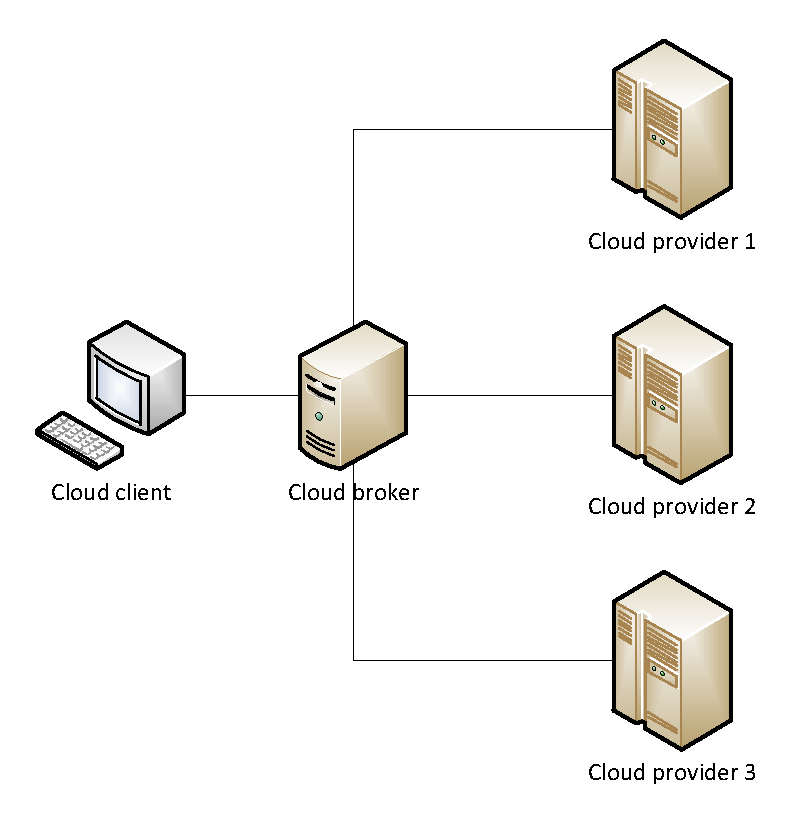
\includegraphics[width=0.6\textwidth]{chapter-7/deployment-cost-physical-nodes}
  \end{center}
  \caption{Deployment cost: environment configuration}
  \label{eval:deployment-cost-physical-nodes}
\end{figure}


\subsection*{Results}
Table \ref{tbl:test-service-deployment-cost-mapping} shows obtained mapping between stacks and cloud providers. Taking into account this result, figure \ref{ch7:service-deployment-cost} shows comparison of cost the client would have to pay with and without such a mapping.

\begin{table}
  \centering
  \begin{tabular}{ c c c  c  }
    \specialrule{.1em}{.05em}{.05em}                  
    & \textbf{CP-1} & \textbf{CP-2} & \textbf{CP-3} \\
    \specialrule{.1em}{.05em}{.05em}                  
    java      & & x & \\ \hline
    ruby      & x & & \\ \hline
    postgres  & & x & \\ \hline
    python    & & & x \\ \hline
    amqp      & & & x \\
    \hline  
  \end{tabular}
  \caption{Chosen cloud providers for the given stack}
  \label{tbl:test-service-deployment-cost-mapping}
\end{table}

\begin{figure}[!ht]
  \begin{center}
    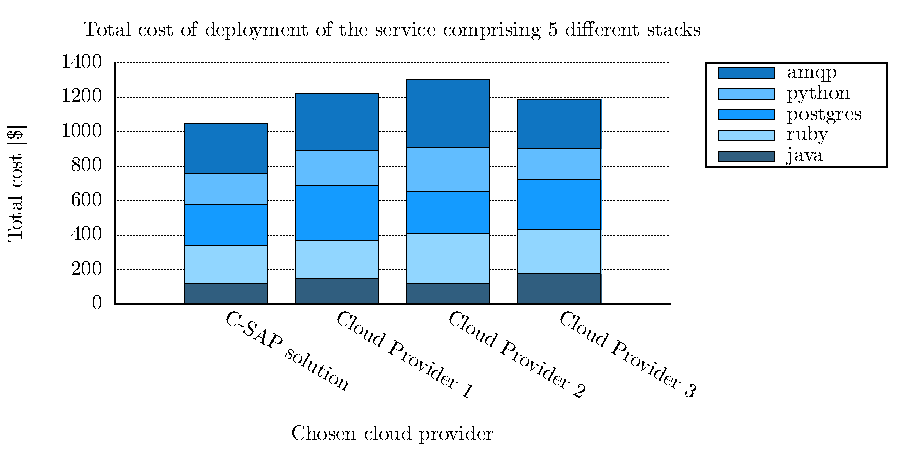
\includegraphics{chapter-7/case-study-service-deployment-reduced-client-costs}
  \end{center}
  \caption{Comparison of the deployment cost when the service is deployed only on a selected cloud provider or a combination of cloud providers selected by Cloud-SAP}
  \label{ch7:service-deployment-cost}
\end{figure}

\subsection*{Conclusion}
Obtained results clearly show that our proof-of-concept product met expectations of this test case as the client was offered the cheapest deployment scheme among various cloud providers for a given software stack.
The mapping mechanism is simple yet considerably powerful -- in this simple scenario the savings were significant since they constituted nearly 20 percent of the price offered by \emph{Cloud Provider 2}. This shows that implementing similar solutions in the real world could be of great benefit to cloud consumers.

\newpage
\section{Auto-scaling -- single-provider based}
\subsection*{Description}
\begin{asparaenum}
\item[\textbf{Motivation}]The aim of this test-case is to show that introducing a multi-layered auto-scaling platform is of a great benefit in terms of cost and resource usage for cloud consumers and cloud providers respectively. What is more, this test should prove that once there are many levels on which scaling operations can be performed, there are significant reduction in costs paid by consumers.
We want to prove it by comparing our proof-of-concept product to \emph{Carina} \cite{Carina}. \emph{Carina} embraces a whole range of various scaling policies for users' environments (environment, in this context, means an application with all its software dependencies that are to be deployed on the cloud), but there is only one way in which they are executed -- by managing the number of virtual machines (i.e. horizontal scaling). Quite on the contrary, \emph{Cloud-SAP} has mechanisms that allow to scale the environment vertically in the first place and if that turns out to be not sufficient, horizontally. This test shows the influence of lack/presence of this feature on price and resource consumption.
\item[\textbf{Scenario}] The test scenario involves
  \begin{inparaenum}[a)]
    \item deployment of a sample environment on the cloud,
    \item substitute the real module responsible for collecting CPU usage date for a mock one,
    \item monitoring the scaling actions performed by each solution,
    \item evaluation of the cost the client has to pay for the service.
  \end{inparaenum}
  Deployment of a service is done in a product-specific manner (up to the point where the vm deployment request is passed to OpenNebula). Mocking the CPU usage was possible by replacing the part in \emph{InformationManager} responsible the collecting CPU data in a host for a request to a web service which generated a time-based mocked-values. Choosing the appropriate function is another issue and is discussed in the next paragraph.
\end{asparaenum}

\subsubsection*{CPU usage function}
We wanted to ensure that both solutions, \emph{Carina} and \emph{Cloud-SAP}, collected the same data regarding the CPU usage for the given time. What is more, the curve should resemble CPU usage in the real business scenarios as much as possible. Thus, we took into account the following factors:
\begin{itemize}
  \item every peak in CPU usage should be followed by a gradual descent which would mimic the real auto-scaling actions executed by each solution,
  \item (boundary conditions) CPU usage should be between 0 and 100 and, additionally, should exceed the previously set scaling threshold value of each solutions so that it would trigger the scaling policies evaluation
  \item once the scaling operations have completed, CPU usage should be constant at a rate which would not introduce any changes in the environment settings (such as the number of virtual machines and parameters of any virtual machine)
\end{itemize}
This resulted in the function whose formula is in \eqref{eq:cpu-mock-usage} and plot in figure \ref{eval:auto-scaling-1cp-cpu-usage-function}.
\begin{eqnarray}
  %f(x) = (1751 *x)/132+(3 *x**2)/8-(31* x**3)/264
  %x <= 11.583 ? f(x) : ( x <= 21.441 ?  f(x - 10) : 25 )
  f(x) &=& -\frac{31}{264}x^3+\frac{3}{8}x^2+\frac{1751}{132}x \nonumber \\
  CPU\_usage(t) &=& \left\{
  \begin{array}{l l l}
    f(t) & \quad 0 & \le t < 11.583 \\
    f(t-10) & \quad 11.583 & \le t < 21.441 \\
    25 & \quad 21.441 & \le  t \\
\end{array} \right.
\label{eq:cpu-mock-usage}
\end{eqnarray}

\begin{figure}[!ht]
  \begin{center}
    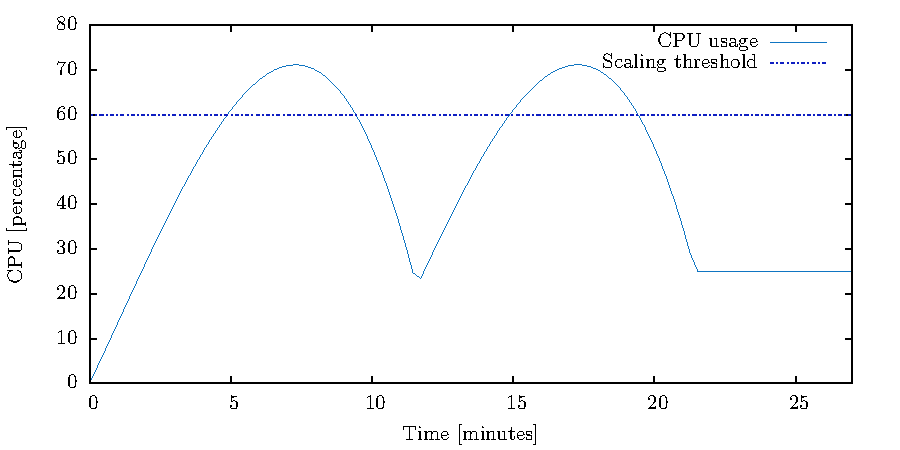
\includegraphics{chapter-7/cpu-usage-mock}
  \end{center}
  \caption{Auto-scaling - single-provider based: CPU usage function}
  \label{eval:auto-scaling-1cp-cpu-usage-function}
\end{figure}

Because \emph{Carina} is capable of only horizontal scaling and \emph{Cloud-SAP} of both horizontal and vertical, one can question whether the descent in CPU usage can be actually the same in both cases. To answer this question we want to look into the description of the virtual machines comprising the deployed environment. It states that each VM can use up to 30\% power of the CPU of a host. Thus, we can be fairly sure that adding another virtual machine that uses 0.3 CPU capacity of its host is equivalent with changing the CPU usage settings of already deployed VM from 30 to 60\%.
\subsection*{Preconditions}
\subsubsection*{Environment specification}
\begin{asparaenum}
  \item[\textbf{Auto-scaling policy specifications}] As it is shown in figure \ref{eval:auto-scaling-1cp-cpu-usage-function}, we set in both products the threshold values of CPU usage that trigger performing auto-scaling actions to 20 and 60 percent. To apply this setting, the auto-scaling part of service specification looks as follows: in Carina the user has to add the parameters of an auto-scaling policy in a hash that describes the environment under key \emph{:elasticy\_policy}. It is possible to specify the minimal and the maximal number of virtual machines that forms the environment and, what is most important, expressions which evaluation results in scaling the application. The part responsible for this is shown in listing \ref{lst:auto-scaling-1cp-carina-service-spec}.\lstinputlisting[caption=Carina service specification used for testing auto-scaling with 1 cloud provider, label=lst:auto-scaling-1cp-carina-service-spec]{auto-scaling-1cp-carina-service-spec} In Cloud-SAP it is a matter of setting appropriate arguments to a specific policy. In this case the policy is \emph{threshold\_model} and values are 20 and 60 for lower and upper bound respectively. The auto-scaling part from service specification is shown in listing \ref{lst:auto-scaling-1cp-cloud-sap-service-spec}. \lstinputlisting[caption=Cloud-SAP service specification used for testing auto-scaling with 1 cloud provider, label=lst:auto-scaling-1cp-cloud-sap-service-spec]{auto-scaling-1cp-cloud-sap-service-spec}
  \item[\textbf{OpenNebula/Carina/Cloud-SAP configuration}] Since Carina and Cloud-SAP used two different instances of OpenNebula installed on separate virtual machines, it is essential the configuration be the same on each of them. Listing \ref{lst:auto-scaling-1cp-one-config} shows the most important OpenNebula excerpt from settings file used in this test case -- polling interval specification, which was set to 30 seconds. To ensure that both products can actually use up-to-date data, they should evaluate their policies every 30 seconds or longer. In Carina the user cannot specify this value, because it is hard-coded in source code to 60 seconds. In Cloud-SAP, however, this value was set in a configuration file and was equal to 60 seconds as well as in Carina. \lstinputlisting[caption=OpenNebula configuration excerpt -- information manager, label=lst:auto-scaling-1cp-one-config]{auto-scaling-1cp-one-config}. Vertical scaling mechanism in \emph{Cloud-SAP} is implemented in a way that causes exponential growth of CPU resources consumption. When there is a need to perform a scaling action on CPU usage, current value is taken and increased by 30\%.
  \item[\textbf{Deployment diagrams}] Deployment diagrams show the placement of each component in both installations. They are shown in figures \ref{eval:auto-scaling-1cp-carina-deployment-diagram} and \ref{eval:auto-scaling-1cp-cloud-sap-deployment-diagram}.

  \begin{figure}[!ht]
    \begin{center}
      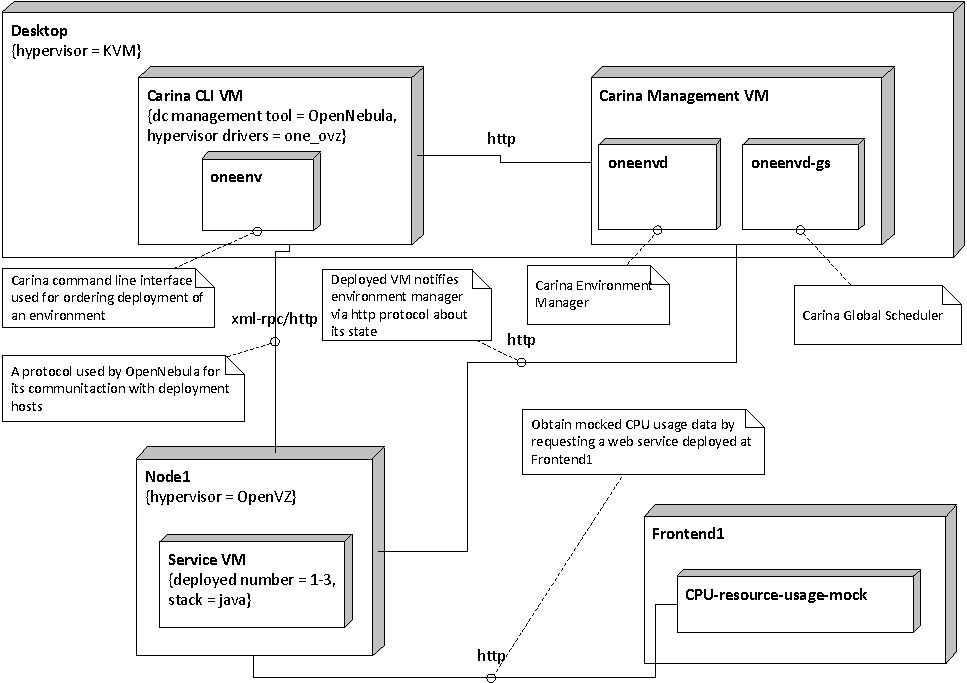
\includegraphics{chapter-7/cpu-usage-carina-deployment-diagram}
    \end{center}
    \caption{Auto-scaling - single-provider based: deployment diagram of Carina}
    \label{eval:auto-scaling-1cp-carina-deployment-diagram}
  \end{figure}

  \begin{figure}[!ht]
    \begin{center}
      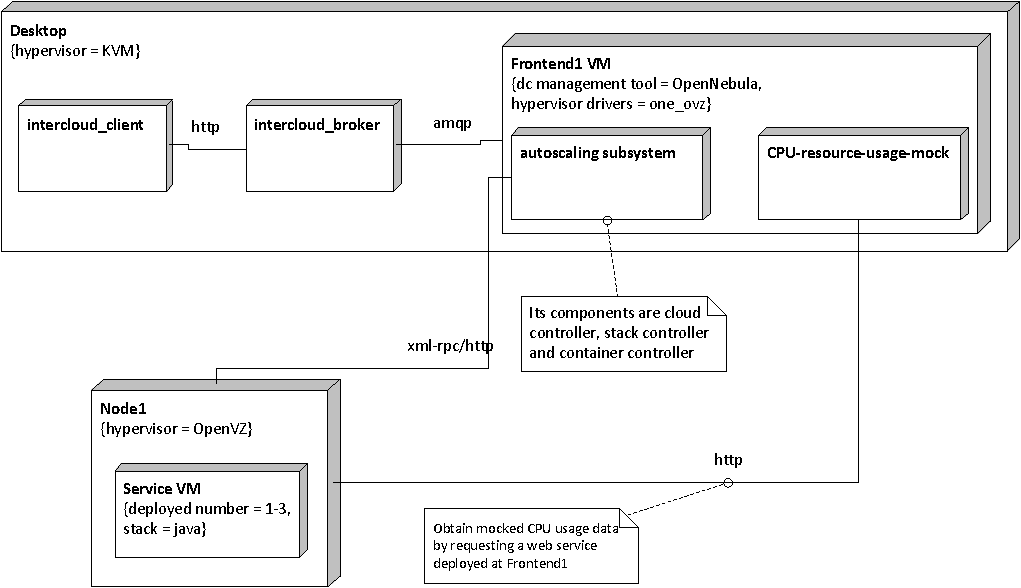
\includegraphics{chapter-7/cpu-usage-cloud-sap-deployment-diagram}
    \end{center}
    \caption{Auto-scaling - single-provider based: deployment diagram of Cloud-SAP}
    \label{eval:auto-scaling-1cp-cloud-sap-deployment-diagram}
  \end{figure}

  \end{asparaenum}

\subsubsection*{Hardware/VM configuration}
All virtual machines were deployed onto \emph{Node1}, which uses \emph{OpenVZ} as a virtualization technology and whose hardware configuration can be found in table \ref{tbl:test-deployment-time-common-hardware-configuration}. \emph{OpenNebula} was installed on a \emph{Frontend1} virtual machine and its configuration is in the same table. \emph{Carina} required the usage of 2 virtual machines which were deployed on \emph{Desktop} with KVM as a hypervisor and whose configuration is in table \ref{tbl:test-auto-scaling-1cp-hardware-configuration}. Diagram \ref{eval:auto-scaling-1cp-physical-nodes} illustrates the physical setup of the test-case. 

\begin{table}
  \centering
  \begin{tabular}{ | l | l | l | l | }
    \hline                        
    Name & CPU & RAM & HD \\
    \hline
    (virtual machine) carina-frontend  & 1 CPU & 1GB & 6GB \\
    (virtual machine) carina-management-vm  & 1 CPU & 1GB & 9GB \\
    \hline  
  \end{tabular}
  \caption{Configuration of hardware/virtual machines used during tests}
  \label{tbl:test-auto-scaling-1cp-hardware-configuration}
\end{table}

\begin{figure}[!ht]
  \begin{center}
    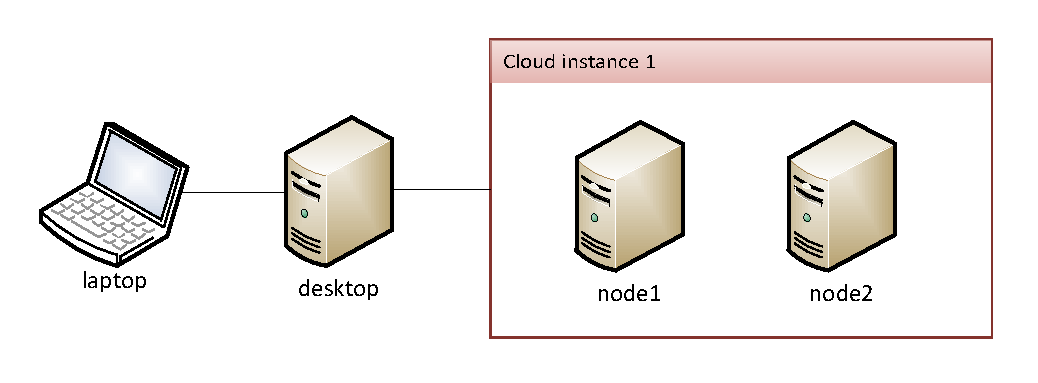
\includegraphics[width=0.8\textwidth]{chapter-7/auto-scaling-1cp-physical-nodes}
  \end{center}
  \caption{Auto-scaling - single-provider based: environment configuration}
  \label{eval:auto-scaling-1cp-physical-nodes}
\end{figure}



\subsection*{Expectations}
As auto-scaling behaviour of both products is determined by CPU usage of the deployed service, we can predict the outcome of the test by thorough analysis of the plot in figure \ref{eval:auto-scaling-1cp-cpu-usage-function}.

The first conclusion is that all auto-scaling actions are performed after exceeding the upper threshold value of CPU usage, this is 60 percent in our case what happens about 5 minutes after the deployment of an environment is completed. CPU consumption remains high for about 2 minutes what enables both products to take appropriate, auto-scaling steps. We expect \emph{Carina} to deploy another virtual machine and \emph{Cloud-SAP} to scale vertically. Then it gradually goes down, which simulates that all taken actions have successfully completed. Then, for another several minutes, the cycle recurs, but this time we expect the proposed solution to scale horizontally. \emph{Carina} is expected to behave as in the previous cycle. Once the cycle has completed, after roughly 21 minutes, the value of CPU consumption remains constant at 25 percent and the test is completed.
\subsection*{Results}
  In the first place it is worth discussing the results of \emph{Carina} and \emph{Cloud-SAP} separately and then compare resource consumption of each solution and its influence on cost paid by the end-user.

\begin{asparaenum}

  \item[\textbf{Cloud-SAP}] Our proof-of-concept solution behaved exactly as expected. To make the discussion more clear, there is an excerpt from a log file of this test run in listing \ref{lst:auto-scaling-1cp-results-csap-logs}. \lstinputlisting[caption=Cloud-SAP logs excerpt regarding auto-scaling actions, label=lst:auto-scaling-1cp-results-csap-logs]{auto-scaling-1cp-results-csap-logs}


\item[\textbf{Carina}] As \emph{Carina} is capable only of horizontal scaling, in discussion of its resource usage we can confine ourselves to counting the number of deployed virtual machines in the given time intervals. In the log files we can trace all actions that were triggered during the test case. As listing \ref{lst:auto-scaling-1cp-results-carina-jobs} shows, they completely met the expectations expressed in the previous section -- there were two ''SCALEUP'' jobs which resulted in increase of the total number of virtual machines comprising the environment.  \lstinputlisting[caption=Carina environment manager logs with taken actions (\emph{jobs}), label=lst:auto-scaling-1cp-results-carina-jobs]{auto-scaling-1cp-results-carina-jobs}. Since the base configuration assumed that the environment consists of 2 virtual machines, we can say that about 10 minutes after deployment of an environment, the number of VMs increased to 3, and after another 10 minutes, to 4.

Deployment finished at 15:25:45 and at this time we started the mock-cpu-usage web service. When the platform concluded that there are insufficient resources, it tried for three times changing parameters (virtual CPU used by the vm) of the virtual machines forming the service. Once scaling vertically was not possible such an information was passed to cloud controller which performed scaling across different cloud providers.
\end{asparaenum}

\subsubsection*{Cost}
In our scenario cost is roughly equivalent with the CPU usage, so the plot of a cost virtually presents the cpu usage. Figure \ref{eval:auto-scaling-1cp-cost-comparison} shows cpu usage by environment when deployed and configured by two competing products.
\begin{figure}[!ht]
  \begin{center}
    \includegraphics{chapter-7/auto-scaling-1cp-cost-comparison}
  \end{center}
  \caption{Auto-scaling - single-provider based: comparison of cost/CPU usage}
  \label{eval:auto-scaling-1cp-cost-comparison}
\end{figure}
If we were to roughly estimate the cost in both solutions it would be equal in Carina:
\begin{equation}
  7\cdot 0.3 + 10\cdot 0.6 + 8\cdot 0.9 = 15.3 \quad \text{[currency unit]}
\end{equation}
and in Cloud-SAP:
\begin{equation}
  7.0166\cdot 0.3 + 2\cdot 0.39 + 2.01667\cdot0.507 + 7.05\cdot 0.659 + 6.91667\cdot 0.959 \approx 15.186483
\end{equation}

\subsection*{Conclusion}
The obtained results shows that the proposed solution has enormous potential in terms of better utilization of available resources of the cloud and reducing cost paid by cloud consumers.

Judging by the plot of cost (figure \ref{eval:auto-scaling-1cp-cost-comparison}), we can be fairly sure that it is possible to obtain better results by proper tuning of the scaling vertical mechanism. In particular, one can consider changing the default CPU growth from 1.3 to other or apply a different strategy, for example a growth by a constant rate. What is more, in order to get the best results, the policy scaling interval must be chosen with a great care with the consideration of specific parameters of a given environment.

\newpage
\section{Auto-scaling -- multiple-provider based}
\subsection*{Description}

\subsubsection{Motivation} This test case aims to prove that scaling across multiple cloud providers is vitally important while ensuring appropriate Quality-of-Service, especially in cases of increased number of service requests. Such scaling scenario, known also as cloud-bursting, leverage benefits arising from offloading application load to an external provider. In order to verify our concept we compare number of transactions per second guaranteed by \emph{Cloud-SAP} and \emph{Carina}. While our proof of concept solution features multi-layer scaling and is cloud federation aware, \emph{Carina} adopts only horizontal scaling. It is expected that test case prove benefits emerging from enriching application platform provider with an cloud federation awareness.
 
\subsubsection{Scenario}
Testing requires following steps to be done:
\begin{enumerate}
\item deploy exemplary service
\item observe system behaviour under load, simulated by a resource usage mock. It is vital for a resource usage to exceed a single provider capabilities
\item assess system characteristics, including number of handled transactions per second
\end{enumerate}

\subsubsection*{Load simulation}
Similarly to a previous test case, we leveraged a resource mock that allows us to precisely control monitoring information returned to an system. Besides, in order to simplify test case, we were solely focused on a CPU usage. CPU usage function has to exceed upper threshold limit at some point and stay at that level, triggering successive auto-scaling events. However, at some point single cloud provider resources will be surpassed. Equation \eqref{eq:cpu-mock-usage-2cp} denotes a resource usage function that is expected to fulfil above-mentioned scenario and is illustrated in figure \ref{eval:auto-scaling-2cp-cpu-usage-function}.
\begin{equation}
 f(x) = \frac{29}{1500}x^3-\frac{21}{20}x^2+\frac{533}{30}x
 \label{eq:cpu-mock-usage-2cp}
\end{equation}

\begin{figure}[!ht]
  \begin{center}
    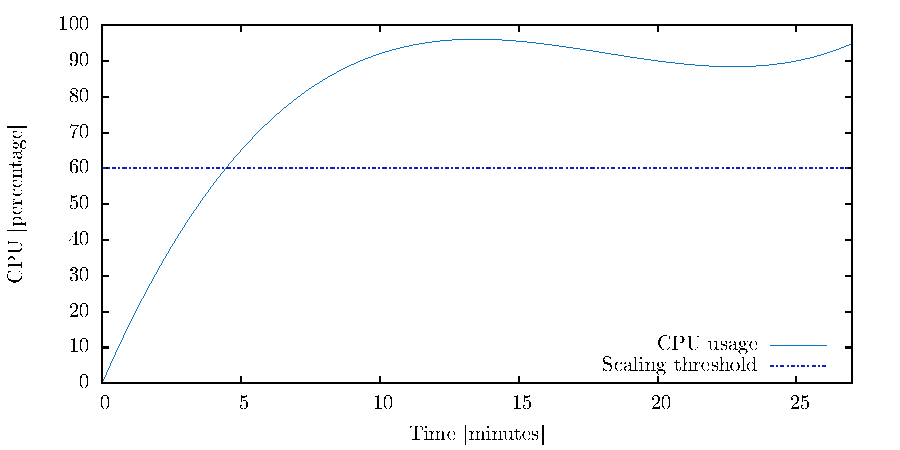
\includegraphics{chapter-7/cpu-usage-mock-multiple}
  \end{center}
  \caption{Auto-scaling - multiple-provider based: CPU usage function}
  \label{eval:auto-scaling-2cp-cpu-usage-function}
\end{figure}

\subsection*{Preconditions}
\subsubsection*{Environment specification}
\begin{asparaenum}
  \item[\textbf{Auto-scaling policy specifications}] Policies used in this test are based on a threshold model with the following properties:
  \begin{itemize}
   \item value below 20 triggers scaling down event
   \item value grater than 60 triggers scaling up event
  \end{itemize}
  However, considering the fact that we are entirely focused on scaling up, only the upper limit is relevant in our case. Listings \ref{lst:auto-scaling-2cp-carina-service-spec} and \ref{lst:auto-scaling-2cp-cloud-sap-service-spec} presents scaling policies for \emph{Carina} and \emph{Cloud-SAP} respectively.
  
  \lstinputlisting[caption=\emph{Carina} service specification used for testing auto-scaling with 2 cloud providers, label=lst:auto-scaling-2cp-carina-service-spec]{auto-scaling-2cp-carina-service-spec}
  \lstinputlisting[caption=\emph{Cloud-SAP} service specification used for testing auto-scaling with 2 cloud providers, label=lst:auto-scaling-2cp-cloud-sap-service-spec]{auto-scaling-2cp-cloud-sap-service-spec}
  
  \item[\textbf{OpenNebula/Carina/Cloud-SAP configuration}] 
  Components common to \emph{Carina} and \emph{Cloud-SAP}, namely \emph{OpenNebula} instances and computing nodes, were configured in the same fashion. Listing \ref{lst:auto-scaling-2cp-one-config} depicts key configuration elements of \emph{OpenNebula} monitoring mechanism.
  
  \lstinputlisting[caption=OpenNebula configuration excerpt -- virtual machine and information manager, label=lst:auto-scaling-2cp-one-config]{auto-scaling-2cp-one-config}
  
  \item[\textbf{Deployment diagrams}] Components that took part during testing are show in figures \ref{eval:auto-scaling-2cp-carina-deployment-diagram} and \ref{eval:autoscale-2cp-cloud-sap-deployment-diagram}.

  \begin{figure}[!ht]
    \begin{center}
      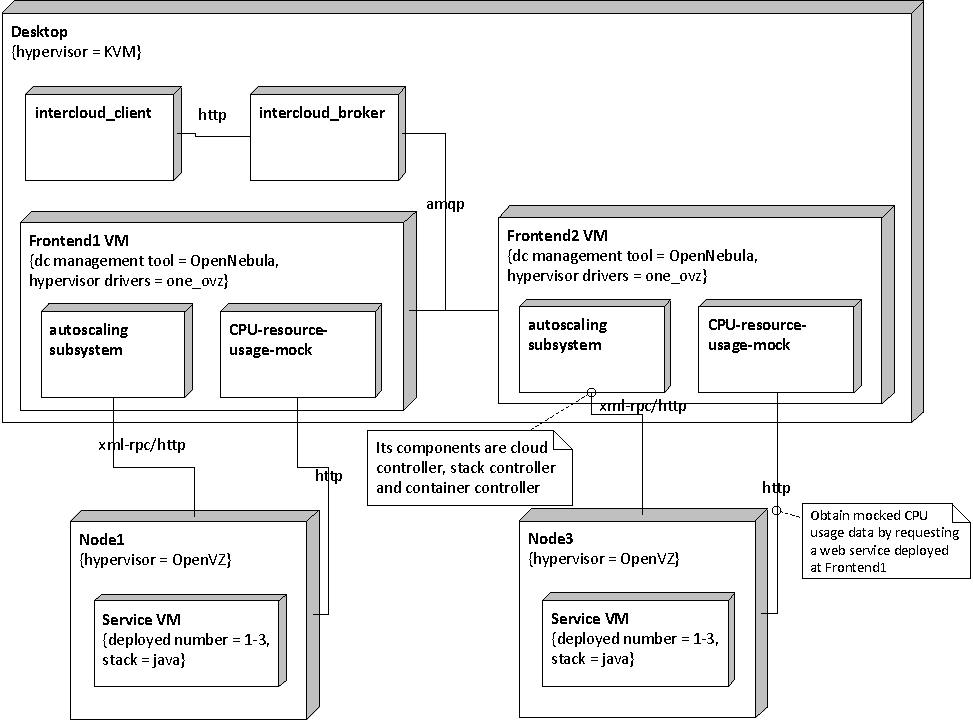
\includegraphics{chapter-7/autoscale-2cp-cloud-sap-deployment-diagram}
    \end{center}
    \caption{Auto-scaling - multiple-provider based: deployment diagram of Carina}
    \label{eval:autoscale-2cp-cloud-sap-deployment-diagram}
  \end{figure}
  
  \begin{figure}[!ht]
    \begin{center}
      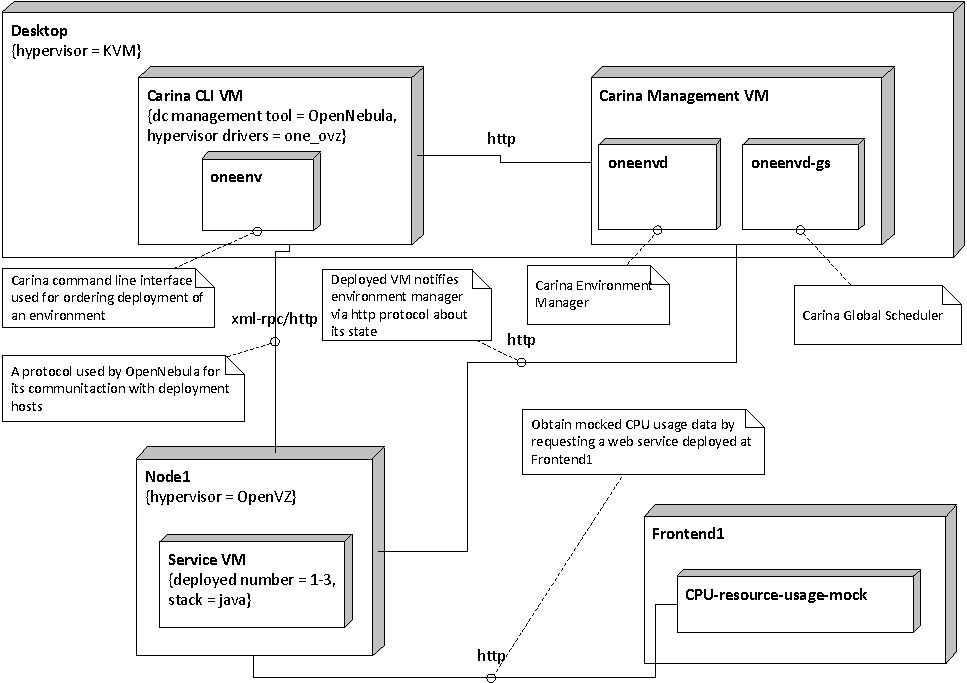
\includegraphics{chapter-7/cpu-usage-carina-deployment-diagram}
    \end{center}
    \caption{Auto-scaling - multiple-provider based: deployment diagram of Carina}
    \label{eval:auto-scaling-2cp-carina-deployment-diagram}
  \end{figure}
\end{asparaenum}

\subsubsection*{Hardware/VM configuration}

Figure \ref{eval:auto-scaling-2cp-physical-nodes} depicts physical configuration of the environment. In short, setup was as follows: all \emph{Cloud-SAP} components, apart from cloud client deployed on \emph{Laptop}, were provisioned on \emph{Desktop}. \emph{Cloud Proivder 1 (CP-1)} is \emph{OpenNebula} instance known as \emph{Frontend1} which uses \emph{Node1} as a computing node and is deployed on \emph{Desktop}, while \emph{CP\-2} uses \emph{Frontend2} and \emph{Node2}. Specification of nodes is listed in table: \ref{tbl:test-deployment-time-common-hardware-configuration}. Deployment cost of a java stack was 50 and 60 using \emph{CP-1} and \emph{CP-2}, respectively.

\begin{figure}[!ht]
  \begin{center}
    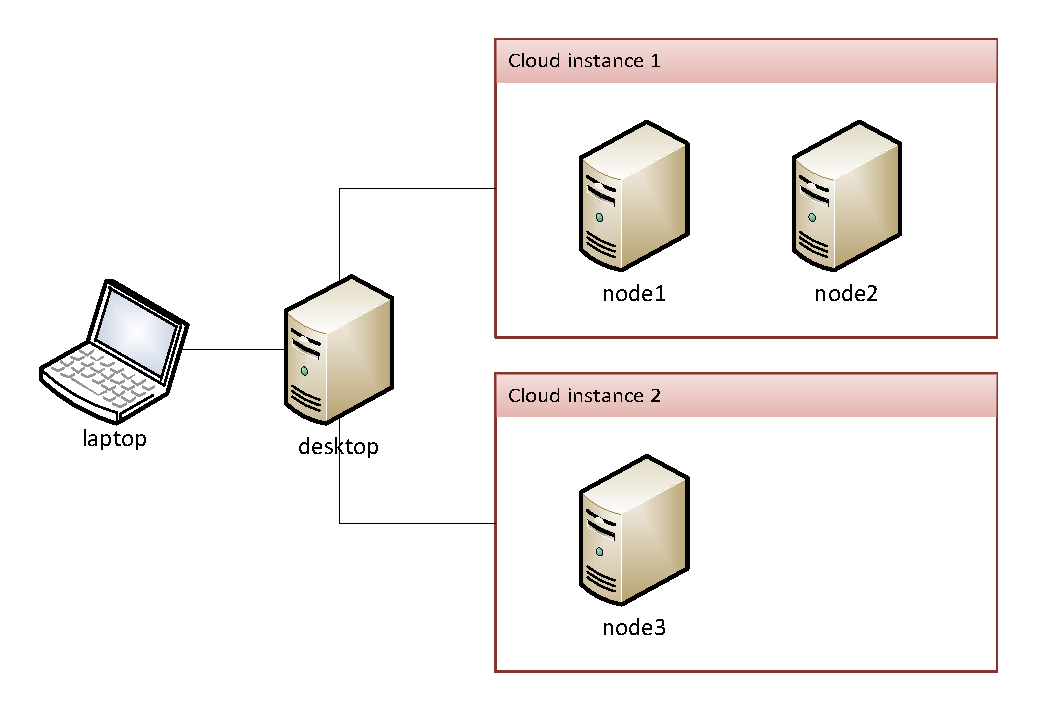
\includegraphics[width=0.7\textwidth]{chapter-7/auto-scaling-2cp-physical-nodes}
  \end{center}
  \caption{Auto-scaling - multiple-provider based: environment configuration}
  \label{eval:auto-scaling-2cp-physical-nodes}
\end{figure}

\subsection*{Expectations}
Taking CPU usage function into account, we can predict outcome of the test. Scaling policy is violated in 5th minute, hence, it is expected that first scaling event occur after that point. Moreover, since that moment, CPU usage remains beyond threshold implying successive scaling actions.

Due to the fact that \emph{Cloud-SAP} favours fine-grained scaling actions such as vertical scaling, it is expected that these actions occur sooner than horizontal scaling. However, at some point \emph{CP-1} capacity won't be sufficient, hence, another stack instance (one master instance, two slaves) will be deployed on \emph{CP-2}. Subsequent scaling actions will take place solely on a \emph{CP-2} 2 and will involve further vertical scaling.

Carina, on the other hand, supports solely horizontal scaling using single cloud provider. On top of that, it is assumed that succeeding slaves instances will be added to a service up to the point where Cloud Provider won't have enough resources to proceed with further scaling requests.

\subsection*{Results}

\begin{asparaenum}

  \item[\textbf{Cloud-SAP}] 
   In total, there were 13 vertical (increasing CPU limit) 2 horizontal (adding a container) scaling events. First action took place minute after first violation of scaling policy rule. Since then, slaves' CPU were successively increasing to the point were further scaling wasn't possible - 13th minute of the test. Therefore, \emph{Cloud-SAP} deployed two new slaves on \emph{CP-2}. Listing \ref{lst:auto-scaling-2cp-results-csap-logs} presents logs covering service lifecycle. \lstinputlisting[caption=Cloud-SAP logs excerpt regarding auto-scaling actions on multiple providers, label=lst:auto-scaling-2cp-results-csap-logs]{auto-scaling-2cp-results-csap-logs}
  
  \item[\textbf{Carina}] 
  Similarly to a \emph{Cloud-SAP}, first scaling event (slave addition) was noticed in 6th minute of test. Scaling jobs were continuously invoked every 2 minutes until capacity of a \emph{CP\-1} hasn been fully exploited. Listing \ref{lst:auto-scaling-2cp-results-carina-jobs} summarises jobs performed by \emph{Carina}. \lstinputlisting[caption=Carina environment manager logs with taken actions (\emph{jobs}), label=lst:auto-scaling-2cp-results-carina-jobs]{auto-scaling-2cp-results-carina-jobs}
\end{asparaenum}
  

\subsubsection*{Transactions per second}
Chart \ref{eval:auto-scaling-2cp-tps-comparison} illustrates how service capabilities changed over the time. Service capability is expressed as a number of transactions per second that can be handled by a service. Please note, that this measure, while giving good insight into application potential, is hard to simulate, hence, we assumed that 1 VCPU provides enough resources to successfully serve 100 TPS. Knowing that, we roughly estimate total service capacity, which at the end of the test amounts to:
\begin{itemize}
 \item Cloud-SAP: 283 transactions per second
 \item Carina: 180 transactions per second
\end{itemize}

\begin{figure}[!ht]
  \begin{center}
    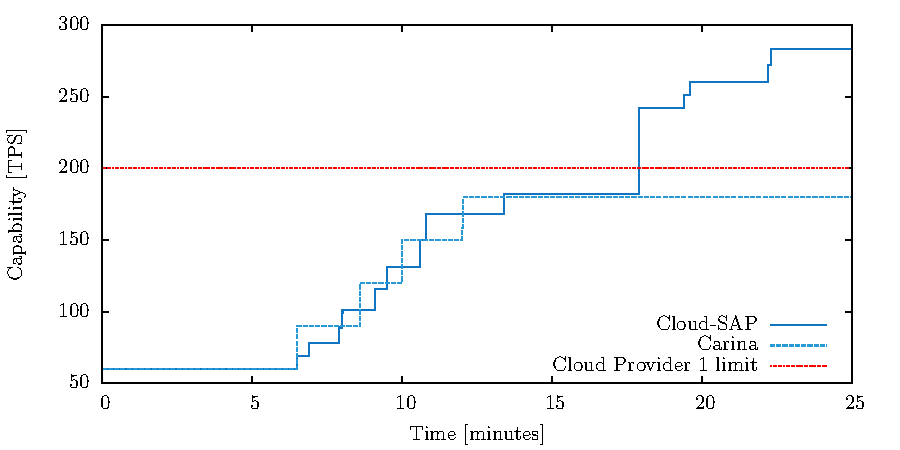
\includegraphics{chapter-7/auto-scaling-2cp-tps-comparison}
  \end{center}
  \caption{Auto-scaling - multiple-provider based: comparison of processed transaction per second}
  \label{eval:auto-scaling-2cp-tps-comparison}
\end{figure}

\subsection*{Conclusion}
Comparing expectations with test output, one can see that expectations has been fully met. While \emph{Carina} was solely focused on horizontal scaling and bound to a single cloud provider, \emph{Cloud-SAP} first took fine-grained actions to later leverage resources of a second cloud provider.

\emph{Cloud-SAP} has been proven to be a better solution, offering greater capabilities to a service. This was possible by exploiting resources of two federated cloud providers, crucial concept behind \emph{Cloud-SAP} design.

\newpage
\section{Deployment time -- solution comparison}
\subsection*{Description}
In this test we want to compare our solution to one of those available at the market which use \emph{OpenNebula} as an underlying tool for managing resources of a data center and \emph{OpenVZ} as a hypervisor in terms of \textbf{deployment time}, one of the most important factors of products whose main purpose is to scale applications.
\emph{Carina} \cite{Carina} can be considered a perfect match of a solution for such a comparison and tests are ran against it.

This test involves the steps of
  \begin{inparaenum}[i)]
    \item instantiating one of the tested product, i.e. Cloud-SAP or Carina,
    \item ordering the deployment of a service whose specification is shown in listing \ref{lst:service-spec-test-deployment-time},
    \item measuring the time needed to set up the environment of the service.
  \end{inparaenum}

\subsection*{Preconditions}
It is assumed that \emph{Cloud-SAP} and \emph{Carina} according with \emph{OpenVZ} as an underlying virtualization technology are correctly installed and configured.
Each test case must be run in an isolation so before performing any test all virtual machines present at the deployment node are removed.
\subsubsection{OpenNebula configuration}
To ensure objectivity in tests, OpenNebula was configured in both products in the same way. One of the key factors that could influence the deployment time is the configuration of scheduler. Its parameters are shown in the listing \ref{lst:one-scheduler-config}.
\lstinputlisting[caption=OpenNebula scheduler configuration, label=lst:one-scheduler-config]{deployment-time-test-sched-config}
\subsubsection{Service description}
The service comprises a simple java enterprise application, deployed in a master-slave configuration with one VM set as a load balancer and other nodes that serve as workers, which uses Tomcat as a web container.

The description of a service expressed in Carina format can be found in listing \ref{lst:carina-config}.

\subsubsection{Hardware configuration}

All virtual machines were deployed on a host named \emph{Node1}, whose configuration can be found in table \ref{tbl:test-deployment-time-common-hardware-configuration}. Diagram presents the physical configuration of nodes.

\begin{figure}[!ht]
  \begin{center}
    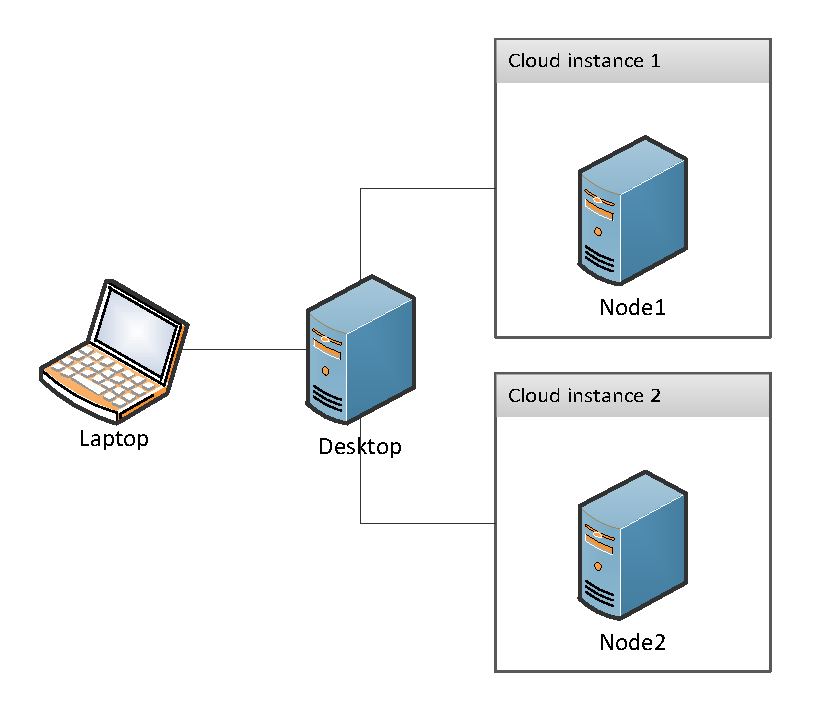
\includegraphics[width=0.6\textwidth]{chapter-7/deployment-time-physical-nodes}
  \end{center}
  \caption{Deployment time - solution comparison: physical environment setup}
  \label{eval:deployment-time-physical-nodes}
\end{figure}

\subsubsection{Environment configuration}
Deployment diagram for \emph{Carina} implementation is shown in figure \ref{ch7:deployment-time-test-deployment-time-carina-deployment-diagram} and for \emph{Cloud-SAP} in figure \ref{ch7:deployment-time-test-cloud-sap-deployment-diagram}.

\begin{figure}[!ht]
  \begin{center}
    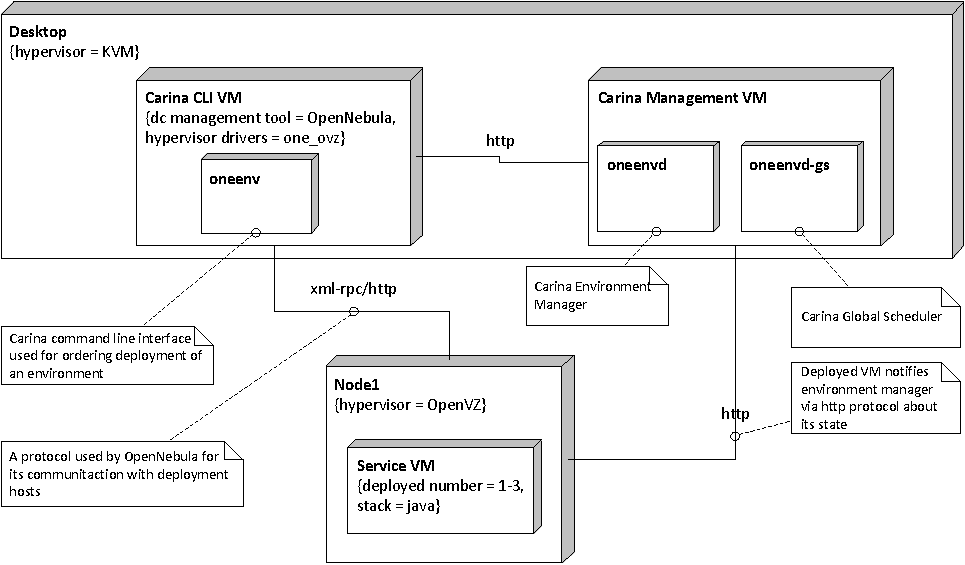
\includegraphics{chapter-7/deployment-time-carina-deployment-diagram}
  \end{center}
  \caption{Deployment diagram of \emph{Carina}}
  \label{ch7:deployment-time-test-deployment-time-carina-deployment-diagram}
\end{figure}

\begin{figure}[!ht]
  \begin{center}
    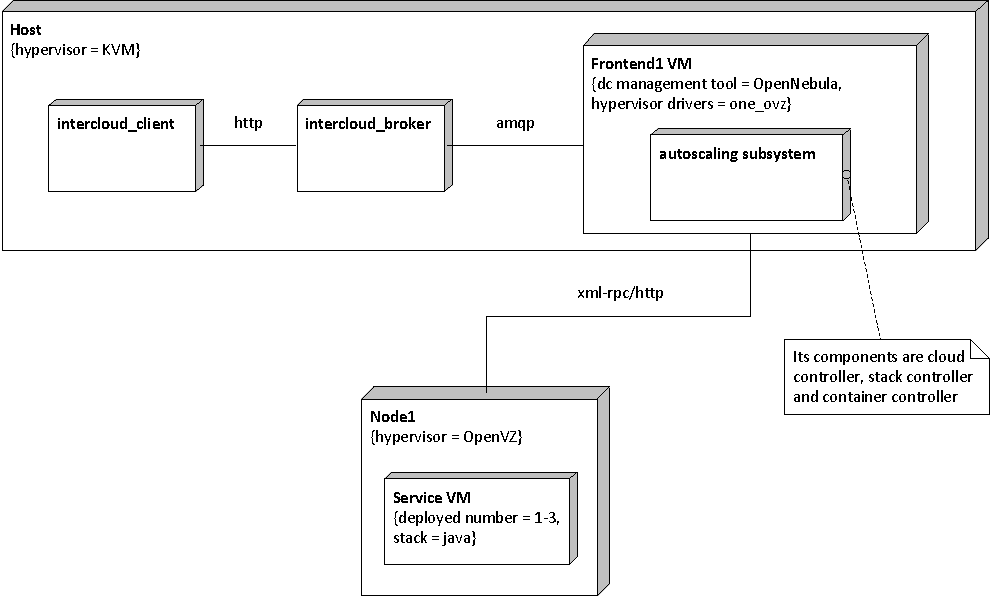
\includegraphics{chapter-7/deployment-time-test-cloud-sap-deployment-diagram}
  \end{center}
  \caption{Deployment diagram of \emph{Cloud-SAP}}
  \label{ch7:deployment-time-test-cloud-sap-deployment-diagram}
\end{figure}

\subsection*{Results}
Obtained results are shown in table \ref{tbl:test-service-deployment-time} and in figure \ref{ch7:deployment-time-test}. For a given number of instances we ordered deploying a service 10 times and the values shown in those figures are an average of these runs.

\begin{table}
  \centering
  \begin{tabular}{ c  c  c }
    \specialrule{.1em}{.05em}{.05em} 
    & \multicolumn{2}{c}{\textbf{Solution}} \\
    \cline{2-3}
    \textbf{Instance no} & Cloud-SAP & Carina \\
    \specialrule{.1em}{.05em}{.05em} 
    2 & 198.0 & 158.7 \\ \hline
    3 & 261.72 & 208.1 \\ \hline
    4 & 294.38 & 230.6 \\
    \hline
  \end{tabular}
  \caption{Average deployment time for the service with the various number of VMs used for the whole environment}
  \label{tbl:test-service-deployment-time}
\end{table}

\begin{figure}[!ht]
  \begin{center}
    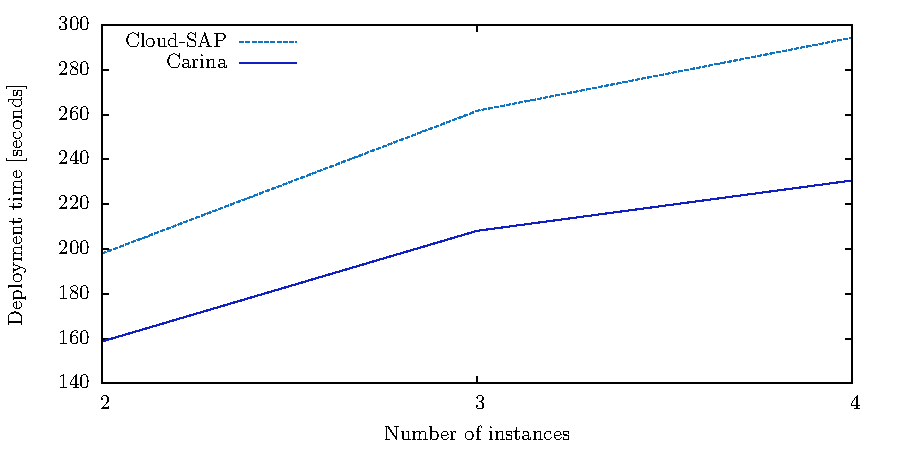
\includegraphics{chapter-7/deployment-time-test}
  \end{center}
  \caption{Average deployment time for two competing products when the variable is the number of instances of VMs}
  \label{ch7:deployment-time-test}
\end{figure}

\subsection*{Conclusion}
As one can can notice, deployment of a java stack takes using \emph{Cloud-SAP} lasts longer than when using \emph{Carina} for the same purpose. Moreover, the more instances are in such stack, the greater difference is. This difference in provisioning time is mainly driven by the fact that \emph{Cloud-SAP} uses a great deal of components in comparison to \emph{Carina}, what is a direct consequence of chosen architecture. Specifically, the request from a client is passed to a broker, then the best provider is chosen and finally the deployment using the select provider and its \emph{Applfow} server takes place. Contrary, \emph{Carina} directly operates on \emph{OpenNebula} giving much simpler flow.

Noticeably, deployment time never was a crucial issue for \emph{Cloud-SAP}, hence, this issue is of a little importance. What is actually important for \emph{Cloud-SAP} is deployment cost and service performance. In other words, slightly greater deployment time is a price that is paid to be sure that resources are deployed optimally and with Quality-of-Service guarantee.
